\documentclass{article}

\usepackage{graphicx,float}

\title{title}
\author{Author}
\date{date}

\begin{document}
\maketitle
\bigskip
\begin{abstract}
To Identify and remove the seasonal component is one of the main issues regarding the time series analysis; and this operation is usually a weel-known affair for national statistical agencies such as Statistics Netherlands. Several procedures are available for this goal, carried out through a wide range of software. Those procedures usually imply the use of filters.  A linear filter is proposed in this paper, which can be incorporated in existing frameworks and packages for the treatment of time series, and which identifies seasonal influences in one step, with no iteration required. The aim of the study is to evaluate the efficacy of this designed filter, using the filtered series as input for a seasonal adjustment procedure, performed by JDemetra+. This latter is a software for time series seasonal adjustment recommended by the ESS and ESCB. It incorporates two methods; X-13-ARIMA, an enhanced X-11 seasonal adjustment procedure (see Dagum, E.B. (1980)), of the U.S. Census Bureau, and TRAMO/SEATS (Gomez, Maravall), of the Bank of Spain. Most of the analysed diagnostics will focus on the spectral analysis.
\end{abstract}
\bigskip
\section{Introduction}
A key concept in traditional time series analysis is the decomposition of a given time series into a trend component, a seasonal component and noise. Seasonality consists in movements repeated throughout the year, with similar intensity in the same period. It means that they are expected to be predictable. Seasonal movements are often large enough that they can mask other characteristics of the data that are of interest to analysts of current trends. Removal of the seasonal component allows to produce series whose movement are easier to evaluate over time. In this manner, is also easier to achieve better forecasts, and to compare trend of different series, once the irregular (noise) component is removed.\\

\begin{figure}[H]
  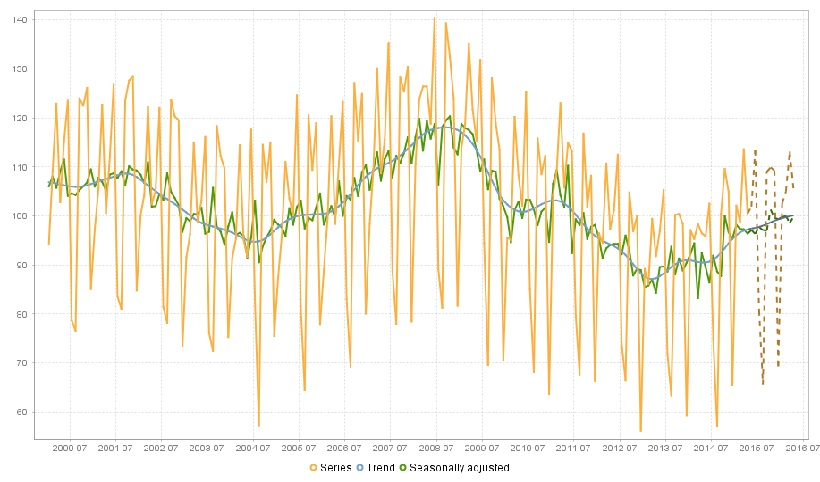
\includegraphics[width=\linewidth]{intro.jpg}
  {\textbf{\scriptsize Figure 1: A decomposition of a time series in trend and seasonally adjusted series performed by JDemetra+.}}
\end{figure}

A common method for obtaining the trend is to use linear filters on given time series, and the simplest class are moving averages with equal weights. It means that the filtered value at time t is an average of the values in a neighbour of pre-defined length of that value. Different adjustment procedures carry out the decomposition of the series through different filters, and most of them have not equal weights. Particularly used are the Henderson filters: a linear smoother developed by Henderson in 1916. It is the most widely applied filter to estimate the trend-cycle component in nonparametric seasonal adjustment software, such as the U.S. Bureau of the Census X-12-ARIMA and its variant, X-13-ARIMA. A good overview of recent developments about capabilities of these softwares is the paper by Findley (2005) and references therein. Those procedures are available also in other software, like Gretl, R, EViews, and, particularly, in JDemetra+. \\
This latter is  a statistical software package for seasonal adjustment supported by Eurostat. It includes two methods: X-13-ARIMA and TRAMO/SEATS. Both of the procedures imply a pre-treatment of the time series, aimed to fit an ARIMA model to the data. Before fitting the model, which will be the starting point for the decomposition of the series, the methods identify variables that have a deterministic effect on the data (like outliers, Easter effects, trading days, leap years etc. etc.), and include those in a regression model  (called RegARIMA). As far as the first step is concerned, the two procedures act really similar, but then they strongly differ in the decomposition part. As mentioned before, X-13-ARIMA works with Henderson smoother, while TRAMO/SEATS estimates the various components, after the pre-treatment, with signal extraction techniques applied to ARIMA models, one for each component of the series. The estimation of the model parameters is done using the so called Weiner-Kolmogorv filters.\\
Another relevant topic related to time series analysis is the revisions problem. Many variables, published at sub-annual frequency (monthly or quarterly), produce new data  continuously. Since the filters used for the decomposition are based on lagged original observation, seasonally adjusted data need to be updated as new observations are available, because to add new values has an impact on the estimates of the components. Those updates are called revisions. A considerable disadvantage of the most used procedures is that revisions produce usually entirely new seasonal adjusted time series. While in practice the updates on older sections of the adjusted time series may be minimal, it is unsatisfactory not to be able to regard any part of the time series as definitive or final. The question is how to reduce the frequency of revisions without losing accuracy in estimation. \\
The paper is structured as follows: the second chapter will discuss the composition of the proposed filter and its properties, evaluating the effect that the set of weights has in the frequency domain and including some concepts about Fourier domain analysis of a time series. Chapter three will report the analysis carried out with a real time series, characterized by a strong seasonal influence. The analysis will focus first on a JDemetra+ seasonal adjustment of the raw series, checking mainly the spectral visualization of the output. Then, data will be adjusted with the proposed set of weights, and the filtered data will be the input for the same JDemetra+ analysis, in order to assess whether the removal of the seasonal component achieved by the filter is satisfactory or not.\\

\end{document}
